\documentclass[12pt,a4paper]{article}
\usepackage[utf8]{inputenc}
\usepackage[spanish]{babel}
\usepackage{graphicx}
\usepackage{hyperref}
\usepackage{geometry}
\geometry{margin=1.5cm}
\usepackage{float}
\usepackage{xcolor}
\usepackage{fancyhdr}

% Encabezado y pie de página
\pagestyle{fancy}
\fancyhf{}
\fancyhead[L]{Calculadora Vectorial}
\fancyhead[R]{Pruebas}
\fancyfoot[C]{\thepage}

\title{\textbf{Archivo de Pruebas - Calculadora Vectorial}}
\author{Bruno Aarón Cruz Rodríguez (TulitasRatchet)\and Mauricio Alejandro Sánchez Ponce (MauAlex1710)}
\date{October 2025}

\begin{document}

\maketitle
\hrule
\vspace{1em}

\section*{Introducción}
Este documento contiene las pruebas realizadas a la Calculadora Vectorial, mostrando la funcionalidad de cada operación, resultados esperados y resultados obtenidos. Todas las visualizaciones están presentadas tanto en 2D como en 3D cuando corresponde.

\section{Datos de prueba}
Se utilizaron los siguientes vectores de ejemplo:

\begin{itemize}
    \item Vector A: $(1, 2, 3)$
    \item Vector B: $(4, 0, -1)$
    \item Vector C: $(2, -1, 5)$
\end{itemize}


\section{Pruebas realizadas}

\subsection{Suma de vectores (A + B)}
\textbf{Resultado esperado:} $(5, 2, 2)$  
\textbf{Resultado obtenido:} $(5, 2, 2)$  

\begin{figure}[H]
    \centering
    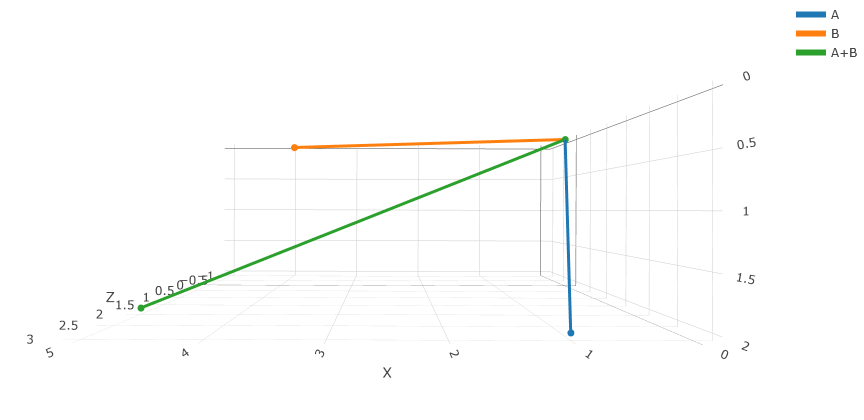
\includegraphics[width=0.7\textwidth]{imagenes/suma_ab.png} % Reemplaza con tu captura
    \caption{Visualización 3D de A + B}
\end{figure}


\subsection{Resta de vectores (A - B)}
\textbf{Resultado esperado:} $(-3, 2, 4)$  
\textbf{Resultado obtenido:} $(-3, 2, 4)$  

\begin{figure}[H]
    \centering
    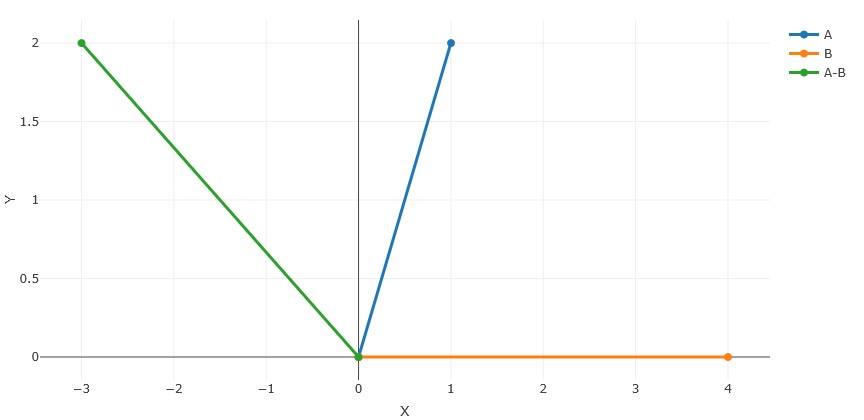
\includegraphics[width=0.7\textwidth]{imagenes/resta_ab.png} % Reemplaza con tu captura
    \caption{Visualización 2D de A - B}
\end{figure}


\subsection{Ángulo entre vectores (A, B)}
\textbf{Resultado esperado:} $~86.28^\circ$  
\textbf{Resultado obtenido:} $~86.28^\circ$  

\begin{figure}[H]
    \centering
    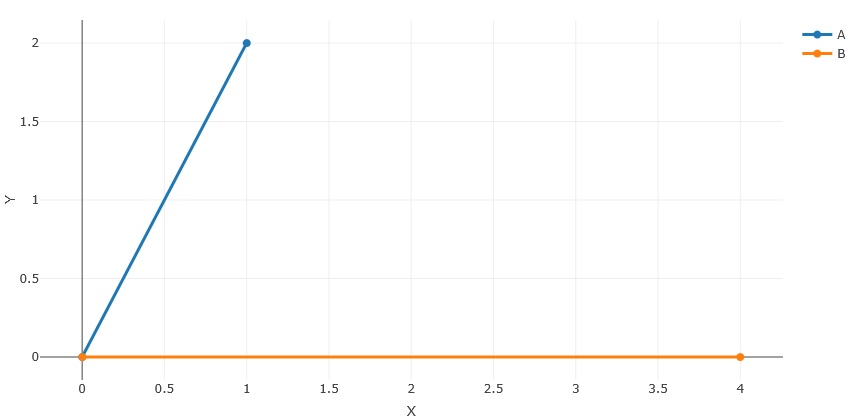
\includegraphics[width=0.7\textwidth]{imagenes/angulo_ab.png} % Reemplaza con tu captura
    \caption{Visualización 2D del ángulo entre A y B}
\end{figure}
\begin{figure}[H]
    \centering
    \includegraphics[width=0.9\textwidth]{imagenes/angulo2_ab.png} % Reemplaza con tu captura
    \caption{Visualización 3D del ángulo entre A y B}
\end{figure}



\subsection{Producto punto (A · B)}
\textbf{Resultado esperado:} $1*4 + 2*0 + 3*(-1) = 1$  
\textbf{Resultado obtenido:} 1
\begin{figure}[H]
    \centering
    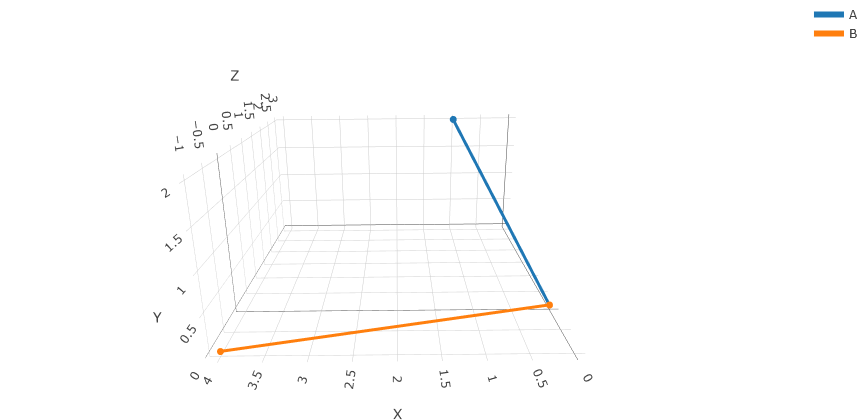
\includegraphics[width=0.7\textwidth]{imagenes/punto_ab.png} % Reemplaza con tu captura
    \caption{Visualización 3D del producto punto entre A y B}
\end{figure}


\subsection{Producto cruz (A × B)}
\textbf{Resultado esperado:} $(2, 13, -8)$  
\textbf{Resultado obtenido:} $(2, 13, -8)$  

\begin{figure}[H]
    \centering
    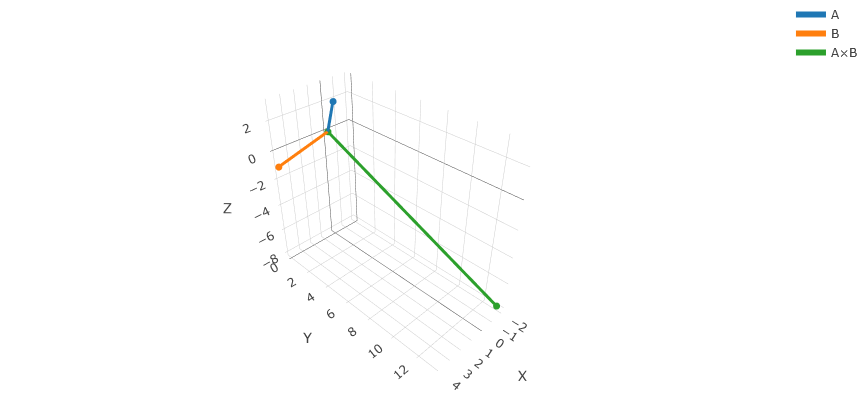
\includegraphics[width=1\textwidth]{imagenes/cruz_ab.png} % Reemplaza con tu captura
    \caption{Visualización del producto cruz A × B}
\end{figure}


\subsection{Producto triple escalar (A · (B × C))}
\textbf{Resultado esperado:} $-57.00$  
\textbf{Resultado obtenido:} $-57.00$ 
\begin{figure}[H]
    \centering
    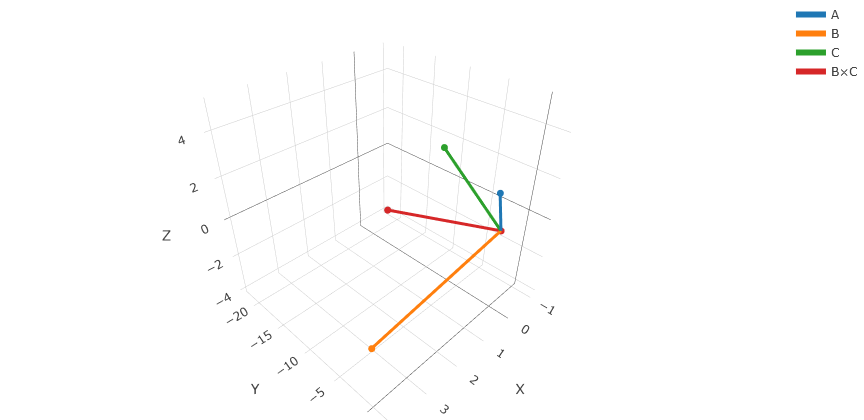
\includegraphics[width=1\textwidth]{imagenes/triple_ab.png} % Reemplaza con tu captura
    \caption{Visualización del producto cruz A × B}
\end{figure}

\subsection{Producto triple vectorial I}
\textbf{A × (B × C)}  
\textbf{Resultado esperado:} $(58, 1, -20)$  
\textbf{Resultado obtenido:} $(58, 1, -20)$  

\begin{figure}[H]
    \centering
    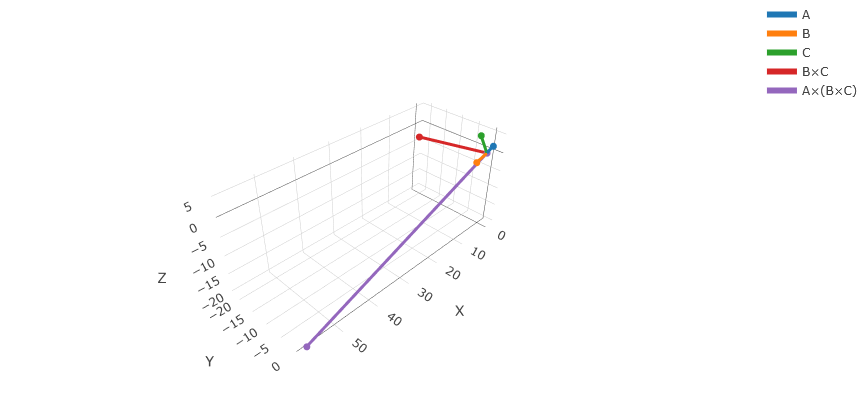
\includegraphics[width=1\textwidth]{imagenes/triple_vectorial.png} % Reemplaza con tu captura
    \caption{Visualización del triple vectorial}
\end{figure}


\subsection{Producto triple vectorial II}
\textbf{(A × B) × C}  
\textbf{Resultado esperado:} $(57, -6, -24)$  
\textbf{Resultado obtenido:} $(57, -6, -24)$  

\begin{figure}[H]
    \centering
    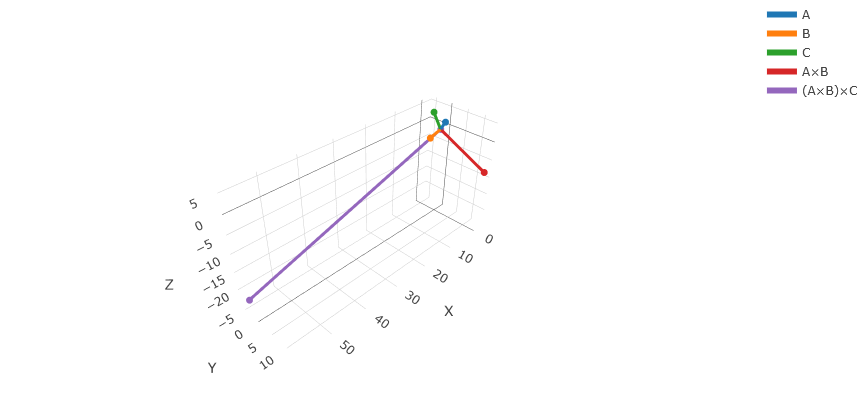
\includegraphics[width=1\textwidth]{imagenes/triple_vectorial2.png} % Reemplaza con tu captura
    \caption{Visualización del triple vectorial}
\end{figure}

\subsection{Angulo con vector (0,0,0)}
\textbf{A, B}  
\textbf{Resultado esperado:} $ERROR$  
\textbf{Resultado obtenido:} $ERROR$  

\begin{figure}[H]
    \centering
    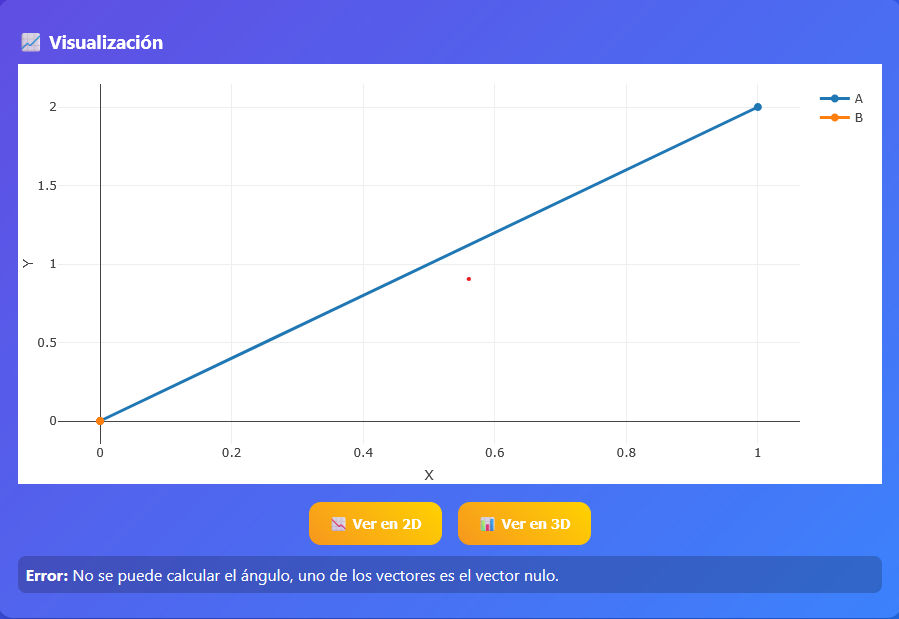
\includegraphics[width=0.7\textwidth]{imagenes/error.png} % Reemplaza con tu captura
    \caption{Visualización de error}
\end{figure}

\subsection{Grafica con todos los vectores en (0,0,0)}
\textbf{A, B}  
\textbf{Resultado esperado:} $(0,0,0)$  
\textbf{Resultado obtenido:} $(0,0,0)$  
\textbf{En todas las operaciones nos deberia de dar (0,0,0)}

\begin{figure}[H]
    \centering
    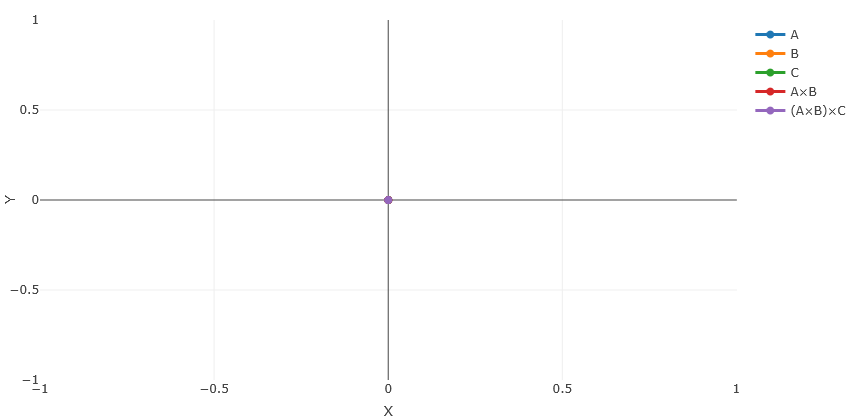
\includegraphics[width=0.7\textwidth]{imagenes/0.png} % Reemplaza con tu captura
    \caption{Visualización (0,0,0)}
\end{figure}


\section*{Conclusiones}
- La Calculadora Vectorial cumple con todas las operaciones implementadas.  
- Los resultados obtenidos coinciden con los resultados esperados de las pruebas.  
- La visualización en 2D y 3D facilita la comprensión de las operaciones vectoriales.

\end{document}
